\section{Linear Algebra}

First of all, a function to properly print vectors and matrices could come in handy. This can be realized the following way:

\begin{lstlisting}[caption=Functions to properly print vectors and matrices]
def getNumberString(pNumber, strLength):
	nStr = str(round(pNumber, 2));
	
	if pNumber >= 0: nStr = " " + nStr;
	
	spacesBefore = strLength - len(nStr);
	
	if spacesBefore > 0:
		for i in range(spacesBefore): nStr = " " + nStr;
	
	return nStr;

def printVector(pVector):
    for element in pVector:
		print(getNumberString(element, 7));

def printMatrix(pMatrix):
	for row in pMatrix:
		rowStr = "";
		for element in row:
			rowStr += getNumberString(element, 7) + " ";
		print(rowStr);
\end{lstlisting}


\subsection{Problem 1.1}


\begin{figure}[!ht]
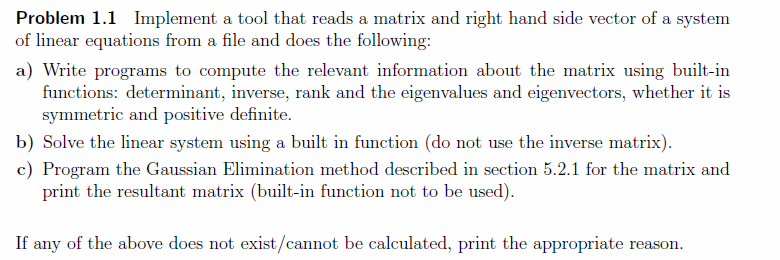
\includegraphics[width=1\textwidth]{chapters/images/desc-1-1}
\end{figure}


To read a matrix and a vector from a text file, first a form has to be determined, for example like this:

\begin{lstlisting}
1 -2 3 -4;
4.1 3 1.1 1;
2 4 1 4;
3 4 3 8;
####
6.1 5.2 4.2 3.1;
\end{lstlisting}

The first part is the matrix, where each line represents one row and each element within that row is seperated by a space. After a line of at least one hashtag, the following values are the elements of the vector, again seperated by a single space. If that form is adhered to, the matrix and vector can be read from the text file with the following script:

\begin{lstlisting}[caption=Extracting the matrix and vector from the text file]
def getVectorFromLine(line):
	numbers = [];
	numberString = "";
	for c in line:
		if c == ' ' or c == ';':
			numbers.append(float(numberString));
			numberString = "";
		else:
			numberString += c;
	
	return numbers;

myMatrix = [];
myVector = [];

textFile = open('matrixTextFile.txt', 'r');

readMatrix = True;

for line in textFile:
	if len(line) > 0:
		if line[0] == '#':
			readMatrix = False;
		else:
			vectorRead = getVectorFromLine(line);
			
			if readMatrix: myMatrix.append(vectorRead);
			else: myVector = vectorRead;


print("Matrix from file:");
mylib.printMatrix(myMatrix);

print("Vector from file:");
mylib.printVector(myVector);
\end{lstlisting}

Afterwards, the matrix and vector from the text file can be used as Python arrays, where the vector is a one-dimensional array and the matrix a two-dimensional array, with the single rows in the first dimension.


\subsubsection{a)}

For the built-in functions the Python library \textit{numpy} can be used:

\begin{lstlisting}[caption=Problem 1.1 a)]
import numpy as np;

matrixRows = len(myMatrix);
matrixCols = len(myMatrix[0]);
vectorRows = len(myVector);

isMatrixSquare = matrixRows == matrixCols;
notSquareStr = "matrix is not square";

matrixArr = np.array(myMatrix);
vectorArr = np.array(myVector);

print("determinant:");

if isMatrixSquare:
	detA = np.linalg.det(matrixArr);
	print(detA);
else:
	print(notSquareStr);

print("inverse:");

if isMatrixSquare:
	invA = np.linalg.inv(matrixArr);
	mylib.printMatrix(invA);
else:
	print(notSquareStr);

print("rank:");

rankA = np.linalg.matrix_rank(matrixArr);
print(rankA);

eigenValues = [];
eigenVectors = [];

if isMatrixSquare:
	eigA = np.linalg.eig(matrixArr);
	for eigi in eigA:
		for el in eigi:
			if isinstance(el, np.ndarray):
				eigenVectors.append(el);
			else:
				eigenValues.append(el);
	
	
	print("eigenvalues:");

	for eigenValue in eigenValues:
		print(eigenValue.real);

	print("eigenvectors:");

	for eigenVector in eigenVectors:
		print(eigenVector.real);
	
else:
	print("eigenvalues and eigenvectors");
	print(notSquareStr);

print("is symmetric:");

if isMatrixSquare:
	isSym = (matrixArr.transpose() == matrixArr).all();
	print(isSym);
else:
	print(notSquareStr);

print("is positive definite:");

if isMatrixSquare:
	isPosDef = np.all(np.linalg.eigvals(matrixArr));
	print(isPosDef);
else:
	print(notSquareStr);
\end{lstlisting}

The results are:

\begin{lstlisting}[caption=Result of 1.1 a), keywordstyle=\color{black}]
determinant:
169.2

inverse:
  -0.13    0.43   -0.53    0.15
   0.11   -0.17    0.71   -0.28
   0.29   -0.24     0.3    0.03
  -0.11    0.01   -0.26     0.2

rank:
4

eigenvalues:
8.25668694865
5.18909337619
-0.222890162424
-0.222890162424

eigenvectors:
[-0.31568286  0.44289131  0.61685718  0.61685718]
[ -7.86684467e-05   3.70103040e-01  -4.34768294e-01  -4.34768294e-01]
[ 0.38980754 -0.19285648 -0.40093074 -0.40093074]
[ 0.86509792 -0.79352215  0.10527324  0.10527324]

is symmetric:
False

is positive definite:
True
\end{lstlisting}

Since the matrix in the text file is square all calculations could be done.


\subsubsection{b)}

In order to solve the linear system, it has to be check first whether number of columns in the matrix equals the number of rows in the vector. If so, a built-in function from \textit{numpy} can be used to solve the system:

\begin{lstlisting}[caption=Problem 1.1 b)]
if not isMatrixSquare:
	print(notSquareStr);
	sys.exit();

if matrixCols != vectorRows:
	print("number of matrix columns and vector rows aren't equal");
	sys.exit();

linSolutions = np.linalg.solve(matrixArr, vectorArr);

xNum = 1;

for linSolution in linSolutions:
	print("x" + str(xNum) + " = " + str(linSolution));
	xNum += 1;
\end{lstlisting}

The resulting x values are:

\begin{lstlisting}[caption=Result of 1.1 b), keywordstyle=\color{black}]
x1 = -0.33829787234
x2 = 1.88156028369
x3 = 1.88794326241
x4 = -1.13439716312
\end{lstlisting}


\subsubsection{c)}

The Gaussian Elemination can be realized without an built-in function in the following way:

\begin{lstlisting}[caption=Problem 1.1 c)]
def gaussElemMethod(matrix, vector):
	n = len(matrix[0]);
	
	for k in range(n - 1):
		maxL = -1;
		for l in range(k, n):
			maxL = max(maxL, abs(matrix[l][k]));
		
		mFound = -1;
		
		for m in range(n):
			if abs(matrix[m][k]) == maxL:
				mFound = m;
		
		if mFound > 0 and matrix[mFound][k] == 0:
			print("singular");
			continue;
		
		for i in range(k + 1, n):
			qik = matrix[i][k] / matrix[k][k];
			
			for j in range(0, n):
				matrix[i][j] = matrix[i][j] - qik * matrix[k][j];
			
			vector[i] = vector[i] - qik * vector[k];

gaussElemMethod(myMatrix, myVector);

print("matrix after elimination:");
mylib.printMatrix(myMatrix);

print("vector after elimination:");
mylib.printVector(myVector);
\end{lstlisting}

Applying this function to the matrix and vector from the text file leads to the following results:

\begin{lstlisting}[caption=Result of 1.1 c), keywordstyle=\color{black}]
matrix after elimination:
    1.0    -2.0     3.0    -4.0
    0.0    11.2   -11.2    17.4
    0.0     0.0     3.0   -0.43
    0.0     0.0     0.0    5.04

vector after elimination:
    6.1
 -19.81
   6.15
  -5.71
\end{lstlisting}


\subsection{Problem 1.2}

\begin{figure}[!ht]
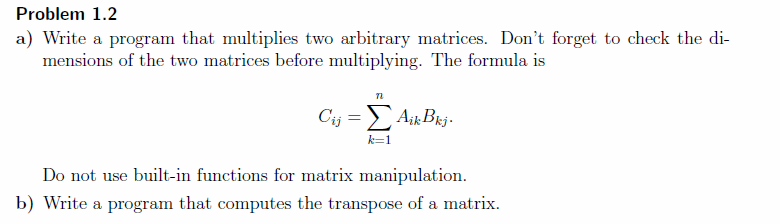
\includegraphics[width=1\textwidth]{chapters/images/desc-1-2}
\end{figure}


\subsubsection{a)}

Multiplying two matrices can be done with the following script:

\begin{lstlisting}[caption=Problem 1.2 a)]
matrix1 = [[1.8, -2], [3, -4.1], [3, 2]];
matrix2 = [[1, -2, -3, 4], [-5, 4, 1, 1]];

print("matrix A:");
mylib.printMatrix(matrix1);

print("matrix B:");
mylib.printMatrix(matrix2);

print("A x B:");

matrix1Rows = len(matrix1);
matrix2Rows = len(matrix2);

matrix1Cols = len(matrix1[0]);
matrix2Cols = len(matrix2[0]);

resultMatrix = [];

if matrix1Cols != matrix2Rows:
	print("number of matrix A columns and matrix B rows aren't equal");

for matrix1Row in range(matrix1Rows):

	resultVector = [];
	for matrix2Col in range(matrix2Cols):
		
		mySum = 0;
		
		for k in range(matrix1Cols):
			mySum = mySum + matrix1[matrix1Row][k] * matrix2[k][matrix2Col];
		
		resultVector.append(mySum);
		
	resultMatrix.append(resultVector);

mylib.printMatrix(resultMatrix);
\end{lstlisting}

The result of the multiplication of the two matrices defined in the script is:

\begin{lstlisting}[caption=Result of 1.2 a), keywordstyle=\color{black}]
matrix A:
    1.8    -2.0
    3.0    -4.1
    3.0     2.0

matrix B:
    1.0    -2.0    -3.0     4.0
   -5.0     4.0     1.0     1.0

A x B:
   11.8   -11.6    -7.4     5.2
   23.5   -22.4   -13.1     7.9
   -7.0     2.0    -7.0    14.0
\end{lstlisting}

\subsubsection{b)}

Transposing a matrix can be done easily with an own function as well:

\begin{lstlisting}[caption=Problem 1.2 b)]
matrix3 = [[1, 2.4], [3.3, -4], [-5, -6.1]];

print("matrix C:");
mylib.printMatrix(matrix3);

matrix3Rows = len(matrix3);
matrix3Cols = len(matrix3[0]);

transposedMatrix = [];

for j in range(matrix3Cols):
	transposedVector = [];

	for i in range(matrix3Rows):
		transposedVector.append(matrix3[i][j]);
	
	transposedMatrix.append(transposedVector);

print("C transposed:");
mylib.printMatrix(transposedMatrix);
\end{lstlisting}

The result is:

\begin{lstlisting}[caption=Result of 1.2 b), keywordstyle=\color{black}]
matrix C:
    1.0     2.4
    3.3    -4.0
   -5.0    -6.1

C transposed:
    1.0     3.3    -5.0
    2.4    -4.0    -6.1
\end{lstlisting}
